% !TeX root = ../main.tex
%
\chapter{Stabilization}
%
%\begin{figure}[H]
%  \hspace{-10pt}
%  \captionbox 
%  {
%    a
%    \label{fig:Edelta_twinSwingAndCatch}
%  }
%  {
%    \hspace{-1cm}
%    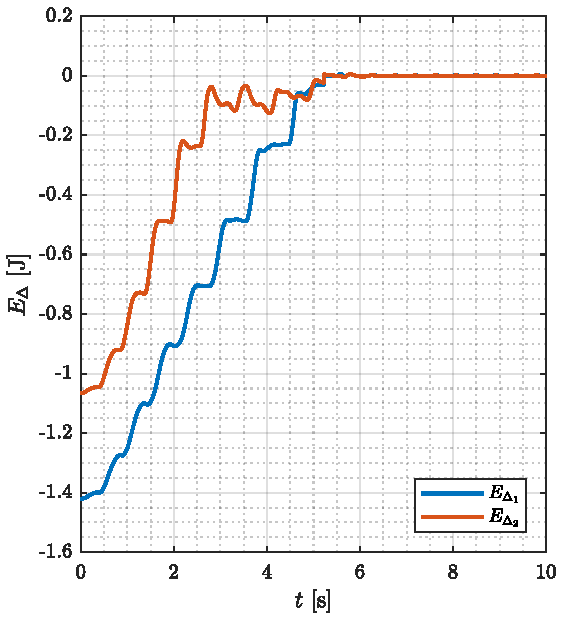
\includegraphics[width=.448\textwidth]{figures/Edelta_twinSwingAndCatch}
%  }
%  \hspace{20pt}
%  \captionbox 
%  {
%    a
%    \label{fig:phase_twinSwingAndCatch}
%  }
%  {
%    \hspace{-1cm}
%    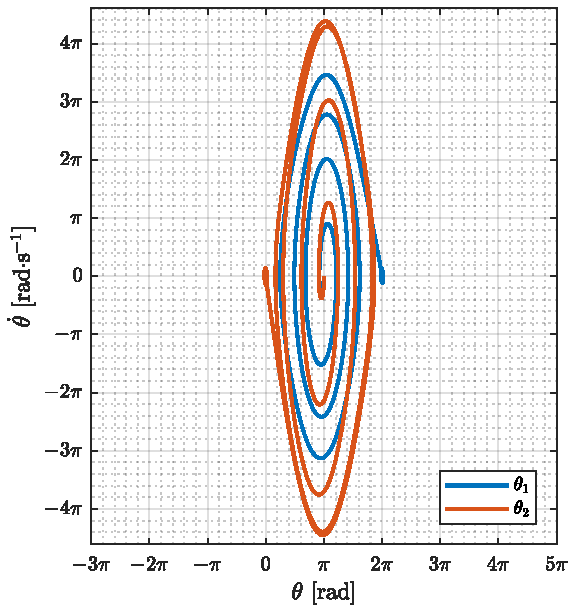
\includegraphics[width=.46\textwidth]{figures/phase_twinSwingAndCatch}
%  }
%\end{figure}
%
In this chapter a Linear Quadratic Regulator (LQR) is designed to stabilize the twin pendulum in upright position taking over from the swing-up controller.\\
The nonlinear state space system from \autoref{eq:nonlinearStateSpaceTwin} are linearized,
\begin{align}
  \vec{A} &= \frac{\partial \vec{f(x)}}{\partial \vec{x}} \whereThree{\vec{x}=\vec{0}\ \ \ \ }{u=0\ \ \ \ }{\text{k}_\text{tanh}=1} \ \ \ , \ \ \
  \vec{B} = \frac{\partial \vec{f(x)}}{\partial u}  \whereThree{\vec{x}=\vec{0}\ \ \ \ }{u=0\ \ \ \ }{\text{k}_\text{tanh}=1} \ \ \ ,
  \label{eq:linearTwin_AB}
\end{align}
\begin{align}
  \vec{A} &= 
  \begin{bmatrix}
    0                         & 0                         & 0 & 1                                                    & 0                                                    & 0 \\
    0                         & 0                         & 0 & 0                                                    & 1                                                    & 0 \\
    0                         & 0                         & 0 & 0                                                    & 0                                                    & 1 \\
    \frac{g (M + m_1)}{M l_1} & \frac{g m_2}{M l_1}       & 0 & -\frac{(M + m_1)(b_{p_1,c} + b_{p_1,v})}{M l_1^2 m1} & -\frac{b_{p_2,c} + b_{p_2,v}}{M l_1 l_2}             & 0 \\
    \frac{g m_1}{M l_2}       & \frac{g (M + m_2)}{M l_2} & 0 & -\frac{b_{p_1,c} + b_{p_1,v}}{M l_1 l_2}             & -\frac{(M + m2)(b_{p_2,c} + b_{p_2,v})}{M l_2^2 m_2} & 0 \\
    \frac{g m_1}{M}           & \frac{g m_2}{M}           & 0 & -\frac{b_{p_1,c} + b_{p_1,v}}{M l_1}                 & -\frac{b_{p_2,c} + b_{p_2,v}}{M l_2}                 & 0
  \end{bmatrix}  \label{eq:linearTwin_A} \\
  \nonumber \\
  \vec{B} &= 
  \begin{bmatrix}
    0  &  0  &  0  &  \frac{1}{M l_1} & \frac{1}{M l_2} & \frac{1}{M}
  \end{bmatrix}^{\mathrm{T}}   \ \ \ .
  \label{eq:linearTwin_B}
\end{align}
%
The controllability and observability matrices are computed for the linearized system,
\begin{align}
  \vec{\mathcal{C}} &= \begin{bmatrix} \vec{B} & \vec{AB} & \vec{A}^2 \vec{B} & \vec{A}^3 \vec{B} & \vec{A}^4 \vec{B} & \vec{A}^5 \vec{B} \end{bmatrix} \Rightarrow  \mathrm{rank}(\vec{\mathcal{C}}) = 6  \label{eq:controllabilityTwin} \\
  \vec{\mathcal{O}} &= \begin{bmatrix} \vec{C} \\ \vec{C}\vec{A} \\ \vec{C}\vec{A}^2 \\ \vec{C}\vec{A}^3 \\ \vec{C}\vec{A}^4 \\ \vec{C}\vec{A}^5 \end{bmatrix} \Rightarrow  \mathrm{rank}(\vec{\mathcal{O}}) = 6  \ \ \ ,
  \label{eq:observabilityTwin}
\end{align}
and since $\vec{\mathcal{C}}$ and $\vec{\mathcal{O}}$ both have full rank, the system is controllable and observable. It is interesting to note that if friction is set to zero and both pendulums are given same length, then $\vec{\mathcal{C}}$ looses rank, that is, the system would no longer be controllable. This is true even if the pendulum masses are different.


minimizing the cost function
\begin{align}
\mathcal{J} &= \int_{0}^{\infty} \vec{x}^T \vec{Q} \vec{x} + \vec{u}^T \vec{R} \vec{u} \ dt \ \ \ .
\label{eq:costFunctionLQR}
\end{align}

Bryson's rule
\begin{align}
  Q_{ii} &= \frac{1}{x_{i,max} }  \ \ \ , \ \ \ \ R_{ii} = \frac{1}{u_{i,max} }
\end{align}
where $x_{i,max}$ are the maximum state errors and $u_{i,max}$ are the maximum inputs.

state-transfer matrix $P$
\begin{align} 
\vec{F} &= -\vec{R}^{-1}\vec{B}^T\vec{P}
\label{eq:gainAndStateTransferMatrix}
\end{align}

%  Abbas Emami-Naeini Gene F. Franklin J. David Powell. ‘Feedback Control of Dynamic Systems’. In: 7th Edition. Pearson, 2015. Chap. 7, pp. 453–585

%  http://www.professeurs.polymtl.ca/jerome.le-ny/teaching/DP_fall09/notes/lec4_LQR.pdf

Algebraic Riccatti equation
\begin{align} 
\vec{A}^T\vec{P}+\vec{P}\vec{A}-\vec{P}\vec{B}\vec{R}^{-1}\vec{B}^T\vec{P}+\vec{Q} &= \vec{0}
\label{eq:algebraicRiccattiEquation}
\end{align}




In this case there is only one input $u$ so $R$ is scalar. The tuned $\vec{Q}$ and $R$ are given by,
\begin{align}
  \vec{Q} &= diag( 1,\ 1,\ \tfrac{1}{ 0.028 },\ 1,\ 1,\ 1 )  \ \ \ , \ \ \ \
  R        = \frac{1}{ 3.3357 } \ \ \ ,
\end{align}

gain vector
\begin{align}
\vec{K} &= [\ 
             \begin{matrix}
               -2742.93 & 2302.58 & 107.09 & -493.15 & 328.26 & 105.18
             \end{matrix}
         \ ]
\end{align}


\begin{figure}[H]
  \hspace{-10pt}
  \captionbox
  {
    a
    \label{fig:theta_twinStabilize}
  }
  {
    \hspace{-1cm}
    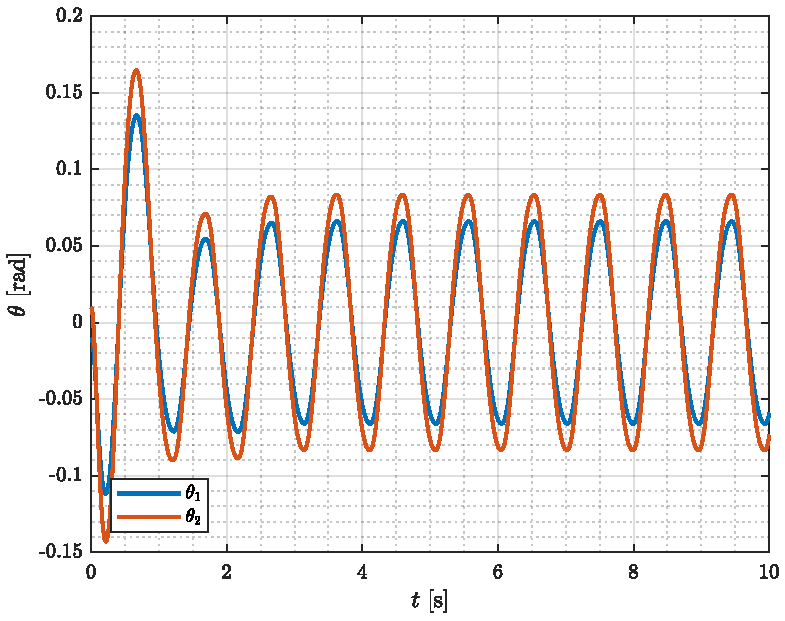
\includegraphics[width=.4\textwidth]{figures/theta_twinStabilize}
  }
  \hspace{20pt}
  \captionbox 
  {
    a
    \label{fig:ia_twinStabilize}
  }
  {
    \hspace{-1cm}
    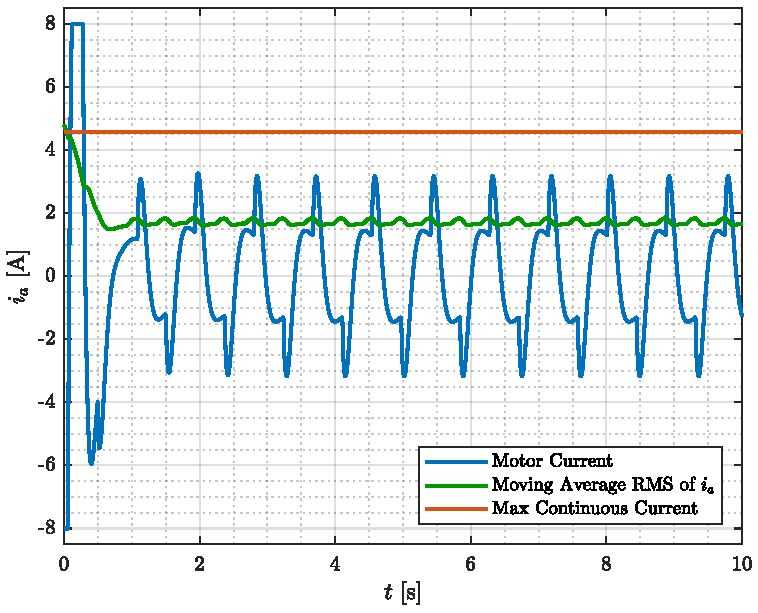
\includegraphics[width=.4\textwidth]{figures/ia_twinStabilize}
  }  
\end{figure}
%
\begin{figure}[H]
  \hspace{-10pt}
  \captionbox
  {
    a
    \label{fig:x_twinStabilize}
  }
  {
    \hspace{-1cm}
    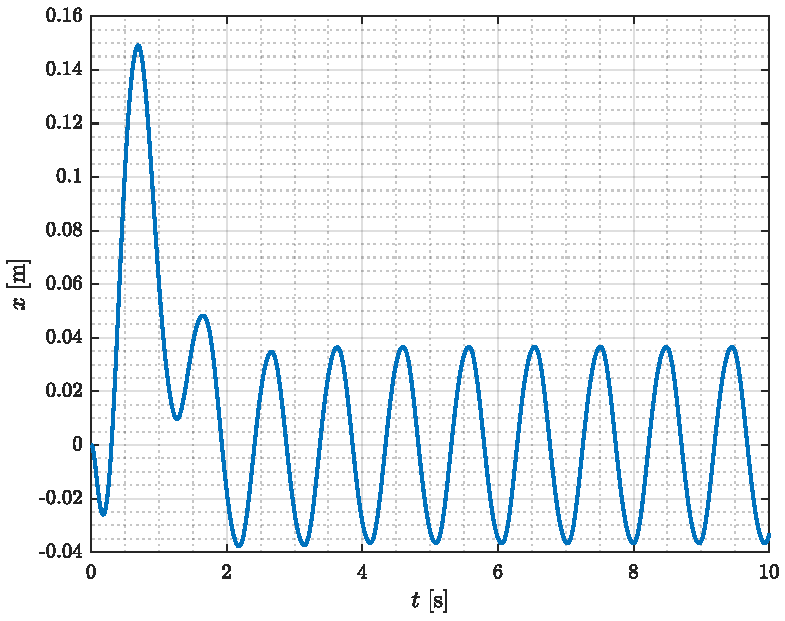
\includegraphics[width=.4\textwidth]{figures/x_twinStabilize}
  }
  \hspace{20pt}
  \captionbox 
  {
    a
    \label{fig:xDot_twinStabilize}
  }
  {
    \hspace{-1cm}
    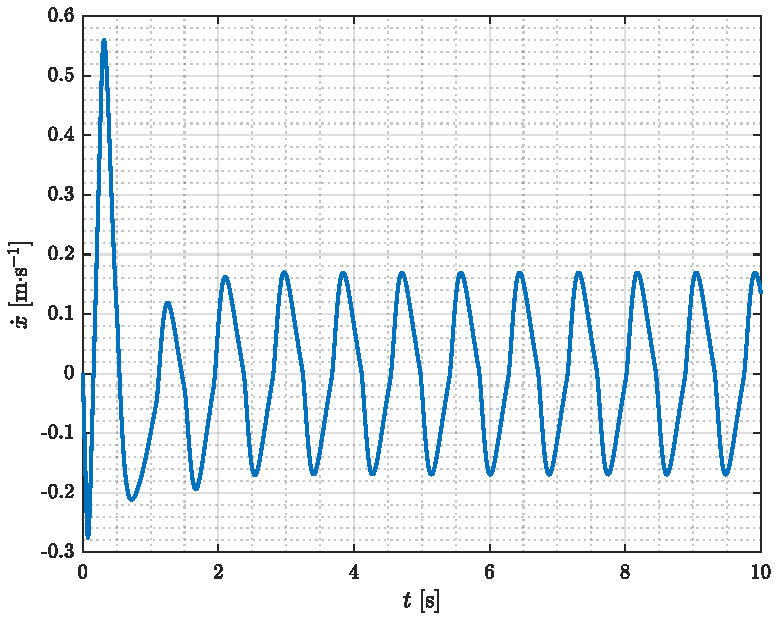
\includegraphics[width=.4\textwidth]{figures/xDot_twinStabilize}
  }  
\end{figure}

























\begin{figure}[H]
  \hspace{-10pt}
  \captionbox 
  {
    a
    \label{fig:theta_twinSwingAndCatch}
  }
  {
    \hspace{-1cm}
    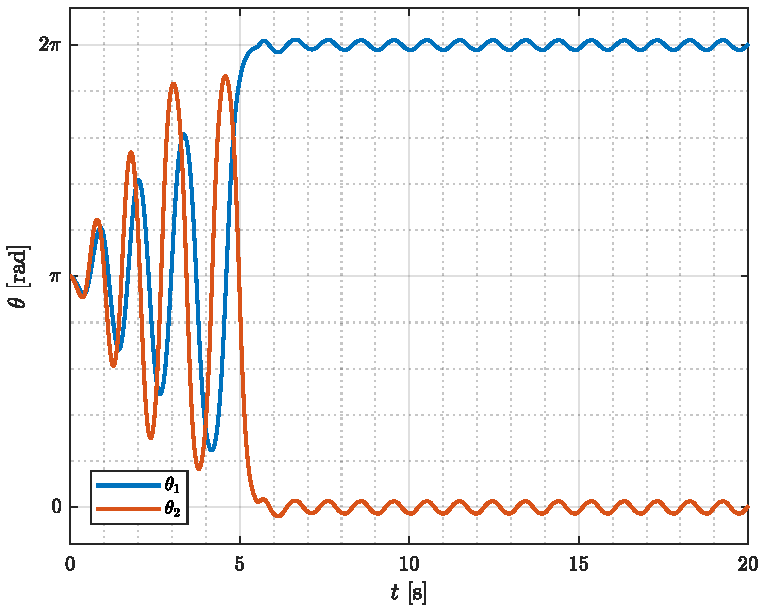
\includegraphics[width=.46\textwidth]{figures/theta_twinSwingAndCatch}
  }
  \hspace{20pt}
  \captionbox 
  {
    a
    \label{fig:ani_twinSwingAndCatch}
  }
  {
    \hspace{-1cm}
    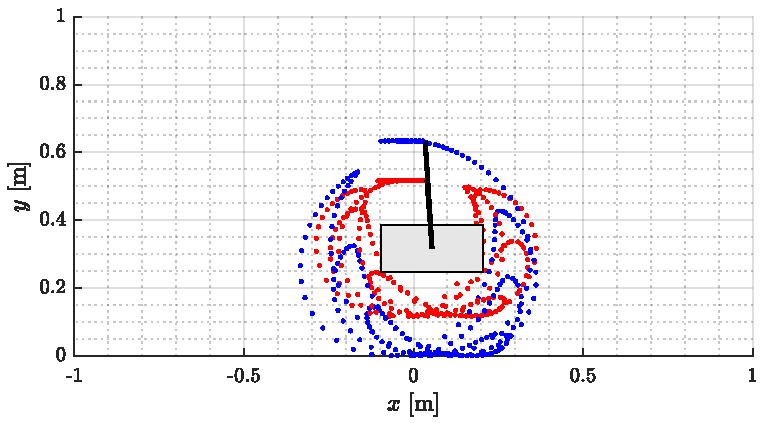
\includegraphics[width=.46\textwidth]{figures/ani_twinSwingAndCatch}
  }
\end{figure}
%
%
\begin{figure}[H]
  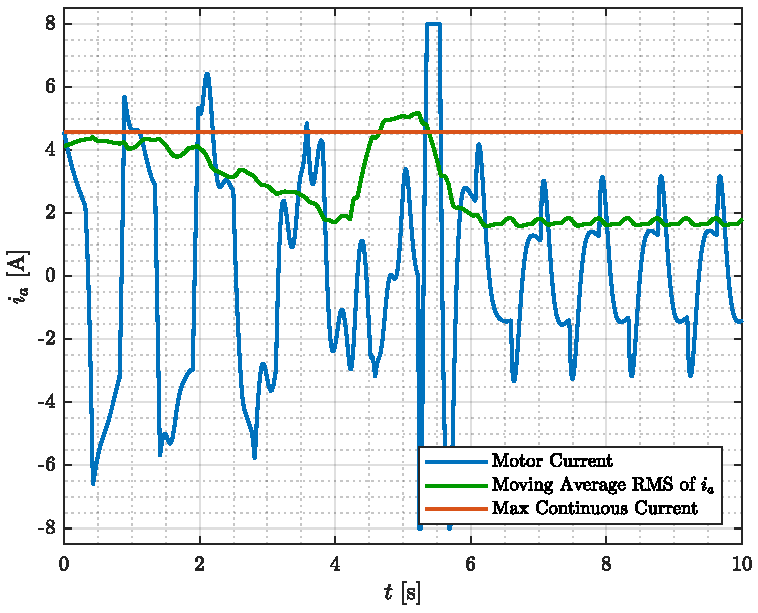
\includegraphics[width=.5\textwidth]{figures/ia_twinSwingAndCatch}
  \caption{a}
  \label{fig:ia_twinSwingAndCatch}
\end{figure}
%
\begin{figure}[H]
  \hspace{-10pt}
  \captionbox
  {
    a
    \label{fig:x_twinSwingAndCatch}
  }
  {
    \hspace{-1cm}
    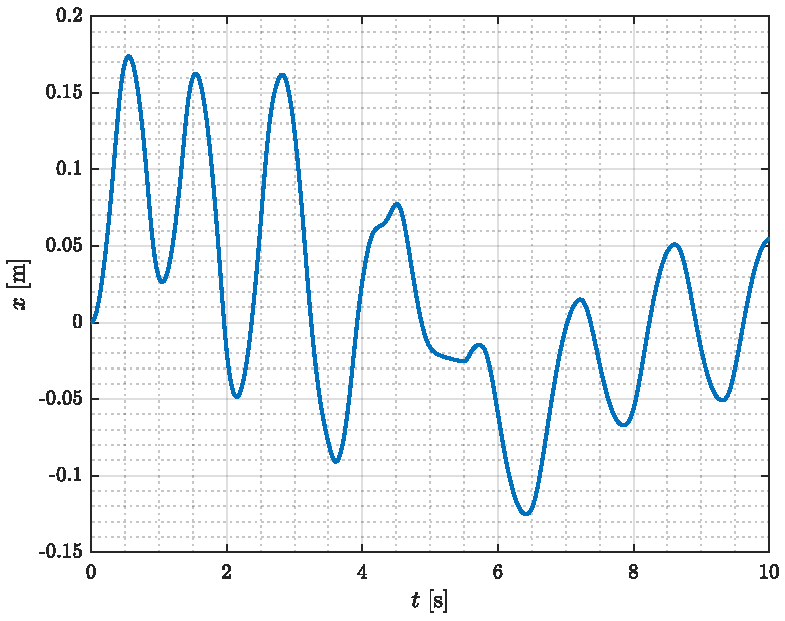
\includegraphics[width=.4\textwidth]{figures/x_twinSwingAndCatch}
  }
  \hspace{20pt}
  \captionbox 
  {
    a
    \label{fig:xDot_twinSwingAndCatch}
  }
  {
    \hspace{-1cm}
    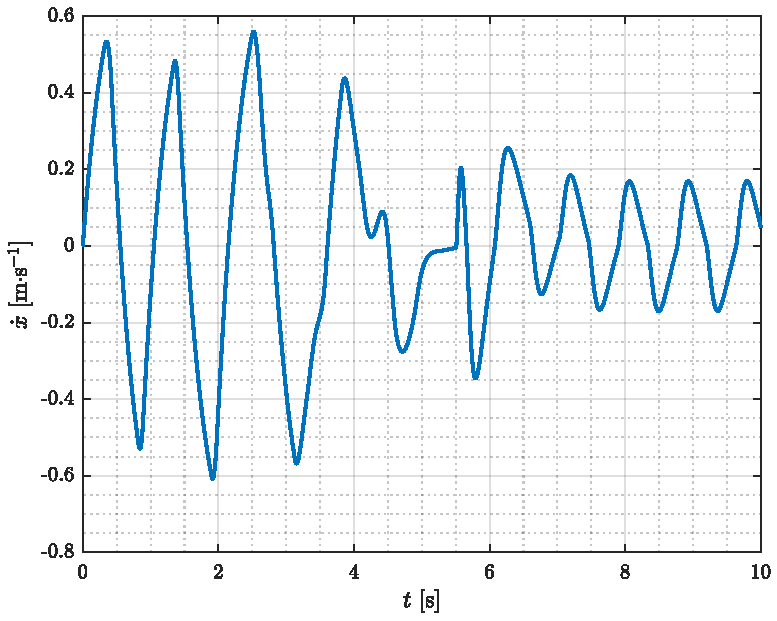
\includegraphics[width=.4\textwidth]{figures/xDot_twinSwingAndCatch}
  }  
\end{figure}
%
%
%\begin{figure}[H]
%  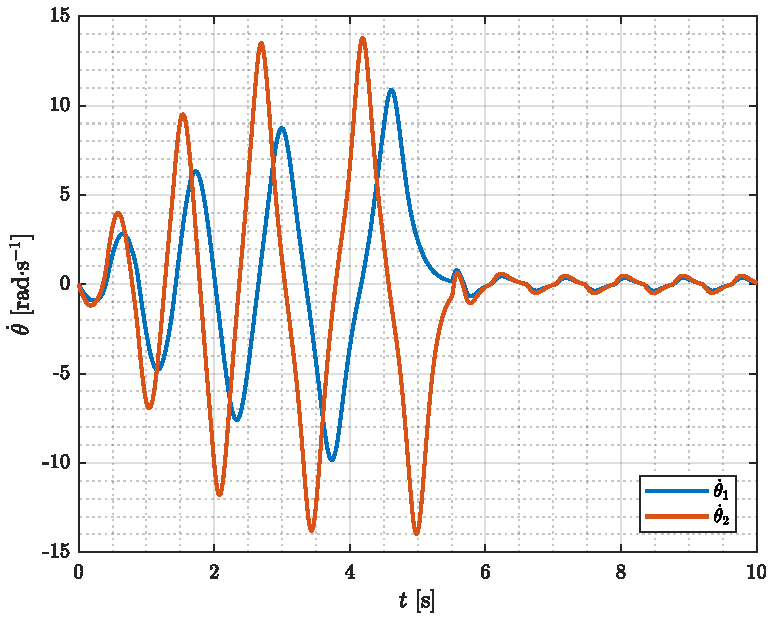
\includegraphics[width=.6\textwidth]{figures/thetaDot_twinSwingAndCatch}
%  \caption{thetaDotTwinSwingAndCatch}
%  \label{fig:thetaDot_twinSwingAndCatch}
%\end{figure}
%\begin{figure}[H]
%  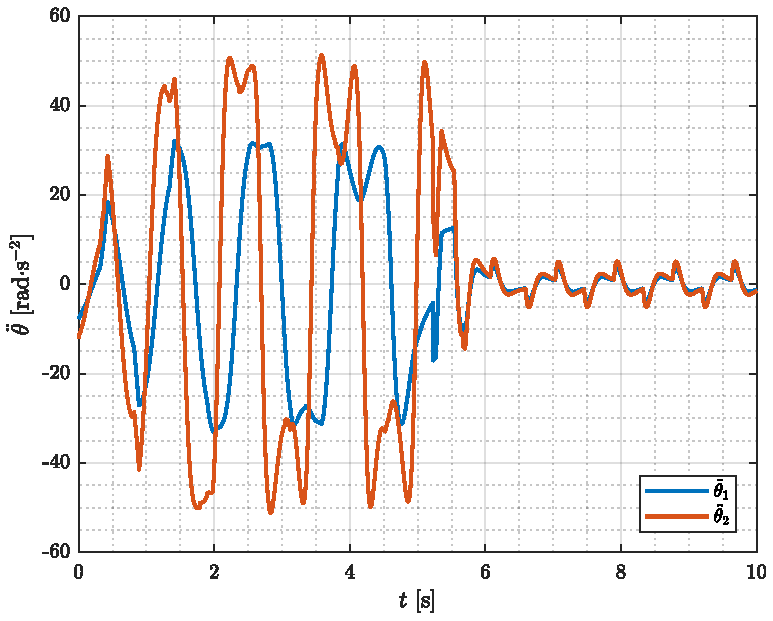
\includegraphics[width=.6\textwidth]{figures/thetaDotDot_twinSwingAndCatch}
%  \caption{thetaDotDotTwinSwingAndCatch}2.
%  \label{fig:thetaDotDot_twinSwingAndCatch}
%\end{figure}
%\begin{figure}[H]
%  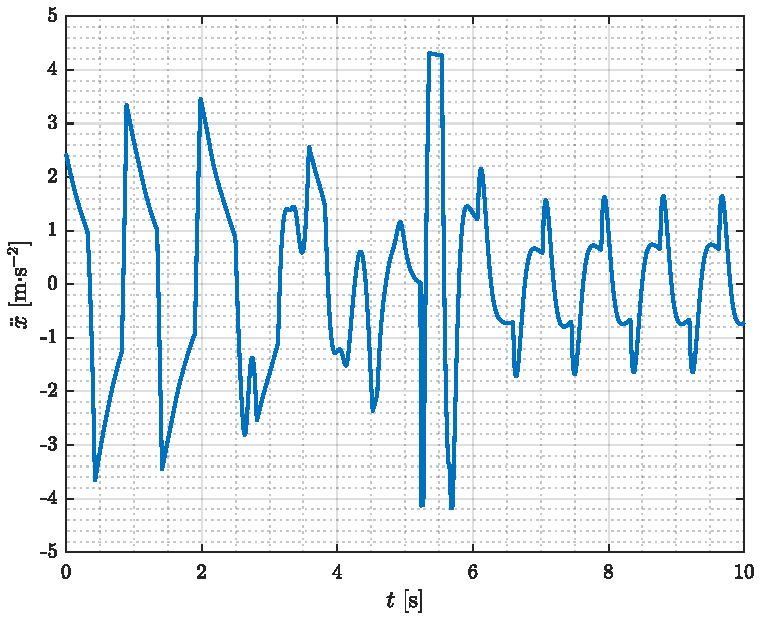
\includegraphics[width=.6\textwidth]{figures/xDotDot_twinSwingAndCatch}
%  \caption{xDotDotTwinSwingAndCatch}
%  \label{fig:xDotDot_twinSwingAndCatch}
%\end{figure}